This section aims to present what objectives the formal analysis is aimed to achieve. Firstly, formal model shall verify the consistency of platform constraints, test special cases and demonstrate relationships among entities through example worlds. \\

%Components of the model, structure and relationship that are defined in the alloy analysis are:
%\begin{itemize}
    %\item User: Abstract signature extended by Student, Company, and University.
    %\item Internship: Represents a professional opportunity with a status that controls its availability.
    %\item Application: Links a Student to an Internship, with a status (Pending, Accepted, Rejected).
    %\item Complaint: Represents an issue raised by a student, resolved by a university, targeting an internship.
    %\item Feedback: Allows students and companies to provide evaluations of internships.
%\end{itemize}

%Constraints:

%Ownership: Internships must have exactly one owning company.
%Unique CVs: Each student must have a unique CV.
%Application Rules: Students can only apply once to the same internship and cannot apply to internships in Draft or Closed states.
%Complaints: Students can only file complaints about internships they were accepted into.
%Feedback Rules: Feedback must target valid internships.




\begin{verbatim}
    // Abstract Signature for Users
    abstract sig User {}
    
    sig Student extends User {
        cv: one CV,
        applications: set Application,
    }
    
    sig Company extends User {
        internships: set Internship,
    }
    
    sig University extends User {
    	monitoredInternships: set Internship
    }
    
    sig CV {}
    
    sig Internship {
        status: one Status
    }
    
    sig Application {
        internship: one Internship,
        status: one ApplicationStatus
    }
    
    sig Complaint {
        filedBy: one Student,
        targetInternship: one Internship,
        resolvedBy: one University
    }
    
    sig Feedback {
        source: one User,
        target: one Internship
    }
    
    abstract sig Status {}
    one sig Active, Closed, Draft extends Status {}
    
    abstract sig ApplicationStatus {}
    one sig Pending, Accepted, Rejected extends ApplicationStatus {}
    
    // Facts to Maintain Consistency
    fact PlatformConstraints {
    
        // Each internship must have one owner
        all i: Internship | one c: Company | i in c.internships
    
        // Each student must have their own unique CV
        all disj s1, s2: Student |
            s1.cv != s2.cv
    
        // Each student must have its own application 
           for a single internship
        all disj s1, s2: Student |
            s1.applications not in s2.applications
    
        // Students can apply to multiple internships, 
            but not the same one twice
        all s: Student |
            all i: Internship |
                lone a: s.applications | a.internship = i
    
        //Each application must have a student
        all a: Application | one s: Student |
            a in s.applications 
    
        // Feedback must only target valid internships
        all f: Feedback |
            f.source in Student + Company and f.target in Internship
    
        // Draft or Closed internships 
           cannot have applicants or complaints
        all i: Internship | (i.status = Closed or i.status = Draft)
            implies no a: Application | a.internship = i
    
        // Each student can only file complaints 
           for internships they were accepted into
        all c: Complaint, s: Student | 
            c.filedBy = s implies some a: s.applications | 
                a.internship = c.targetInternship and a.status = Accepted
    
        // Each student cannot complaint
           for the same internship twice
        all s: Student, i: Internship | lone c: Complaint |
            c.filedBy = s and c.targetInternship = i
    }
    
    pred show [] {
    	#University = 2
    	#Student = 4
    	#Internship = 7
    	#Application = 6
    	#Complaint = 2
    	#Feedback = 1
    
        // Ensure at least one internship is Draft
        some i: Internship | i.status = Draft
    
        // Ensure at least one internship is Closed
        some i: Internship | i.status = Closed
    }
    
    
    run show for 10

    
\end{verbatim}


 \begin{figure}[H]
    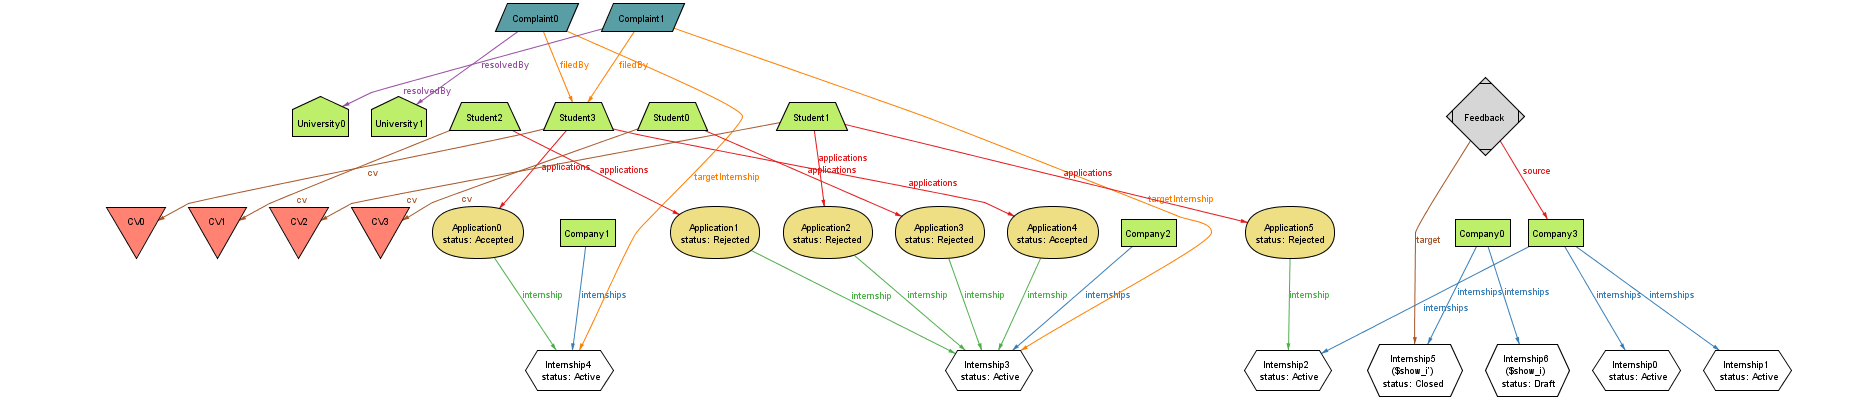
\includegraphics[width=\textwidth,height=\textheight,keepaspectratio]{RASD-Latex/assets/alloyWorld.png}
    \caption{Example world}
    \label{fig:DataRequest}
\end{figure}